% !TEX program = pdflatex
\documentclass[11pt,a4paper]{article}

% --- Page margins and paragraphs ---
\usepackage[margin=1in]{geometry}
\usepackage{parskip}

% --- Basic math and typesetting ---
\usepackage{amsmath,amssymb,amsthm}
\usepackage{xcolor} %

% --- Theorem and definition environments ---
\theoremstyle{definition}
\newtheorem{definition}{Definition}
\newtheorem{example}{Example}

\theoremstyle{plain}
\newtheorem{theorem}{Theorem}
\newtheorem{proposition}{Proposition}
\newtheorem{lemma}{Lemma}

\usepackage{mathtools,booktabs,enumitem,graphicx,url}
\usepackage[hidelinks]{hyperref}
\setlength{\emergencystretch}{2em}
\setlist{topsep=4pt,itemsep=3pt,parsep=0pt}
\raggedbottom
\newcommand{\dd}{\,\mathrm{d}}
\newcommand{\C}{\mathbb{C}}

\begin{document}

% ==================================================
% Title and author information
% ==================================================
\begin{center}
    {\LARGE \textbf{Mathematics Method for Physics--Lecture 8}} \\[0.6em]
    {\large Complex Series: Preliminaries: Exercises}
\end{center}

\vspace{-0.5em}
\noindent\rule{\textwidth}{0.5pt}
\vspace{0.3em}

\begin{center}
    Instructor: Zhaolong Han, SOCE, Shanghai Jiao Tong University;
\end{center}

\vspace{-0.6em}
\noindent Email: han.arkey@sjtu.edu.cn

\vspace{0.4em}
\noindent\rule{\textwidth}{0.5pt}

\vspace{0.8em}

The contour-integral practice and a worked Taylor expansion from the
25 October notes are collected here. Each contour is counterclockwise
unless another orientation is specified. Assigned exercises and
calculation checks follow the worked examples.

\section{Contour-Integral Exercises}
\subsection{Removing an absolute value on a circle}
Evaluate
\begin{equation}\label{eq:01}
I=\oint_{|z|=2}\frac{e^z}{|z-1|^2}\dd z.
\end{equation}
One approach is to set $z=2e^{\mathrm{i}t}$, $0\leq t\leq2\pi$. A shorter approach uses
$z\bar z=4$ on this particular circle:
\begin{equation}\label{eq:02}
|z-1|^2=(z-1)(\bar z-1)
 =(z-1)\left(\frac4z-1\right)
 =-\frac{(z-1)(z-4)}z.
\end{equation}
Consequently,
\begin{equation}\label{eq:03}
I=-\oint_{|z|=2}\frac{z e^z/(z-4)}{z-1}\dd z
   =-2\pi \mathrm{i}\,\frac{e}{1-4}
   =\boxed{\frac{2\pi \mathrm{i} e}{3}}.
\end{equation}
The numerator $ze^z/(z-4)$ is holomorphic on and inside this circle, so
Cauchy's integral formula applies. The replacement $\bar z=4/z$ is an
identity on the contour; it is not an identity throughout the plane.

\subsection{The distinction between \texorpdfstring{$\dd z$ and $|\dd z|$}{dz and |dz|}}
Consider the two different integrals
\begin{equation}\label{eq:04}
I_1=\oint_{|z|=2}\frac{\dd z}{|z-1|^2},
 \qquad
 I_2=\oint_{|z|=2}\frac{|\dd z|}{|z-1|^2}.
\end{equation}
The first is a complex contour integral. The same reduction gives
\begin{equation}\label{eq:05}
I_1=-\oint_{|z|=2}\frac{z/(z-4)}{z-1}\dd z
     =\boxed{\frac{2\pi \mathrm{i}}{3}}.
\end{equation}
The second is an integral with respect to arc length, a positive real
quantity. Since $|\dd z|=2\dd t$,
\begin{equation}\label{eq:06}
I_2=2\int_0^{2\pi}\frac{\dd t}{5-4\cos t}.
\end{equation}
Set $\zeta=e^{\mathrm{i}t}$, so $\dd t=\dd\zeta/(\mathrm{i}\zeta)$. Then
\begin{equation}\label{eq:07}
\begin{aligned}
 I_2&=\frac{2}{\mathrm{i}}\oint_{|\zeta|=1}
             \frac{\dd\zeta}{5\zeta-2\zeta^2-2}\\
    &=-\frac{1}{\mathrm{i}}\oint_{|\zeta|=1}
             \frac{\dd\zeta}{(\zeta-\tfrac12)(\zeta-2)}
      =\boxed{\frac{4\pi}{3}}.
\end{aligned}
\end{equation}
Reversing the contour reverses $I_1$ but leaves the arc-length integral
$I_2$ unchanged.

\subsection{Even cosine moments}
For an integer $n\geq0$, introduce
\begin{equation}\label{eq:08}
J_n=\oint_{|z|=1}\left(z+\frac1z\right)^{2n}\frac{\dd z}{z}.
\end{equation}
For every integer $m$,
\begin{equation}\label{eq:09}
\oint_{|z|=1}z^m\dd z=
 \begin{cases}2\pi \mathrm{i},&m=-1,\\0,&m\neq-1.\end{cases}
\end{equation}
In the binomial expansion of $J_n$, the exponent is $2n-2k-1$.
Only $k=n$ contributes, and hence
\begin{equation}\label{eq:10}
J_n=2\pi \mathrm{i}\binom{2n}{n}.
\end{equation}
On the other hand, $z=e^{\mathrm{i}t}$ gives $z+z^{-1}=2\cos t$ and
$\dd z/z=\mathrm{i}\dd t$. Therefore
\begin{equation}\label{eq:11}
\boxed{\int_0^{2\pi}\cos^{2n}t\dd t
   =\frac{2\pi}{2^{2n}}\binom{2n}{n}
   =\frac{2\pi(2n)!}{2^{2n}(n!)^2}.}
\end{equation}

\subsection{Checking all singularities before using Cauchy's formula}
For the small circle centered at $1$, the function $e^{1/z}$ is holomorphic
throughout the enclosed disk, so
\begin{equation}\label{eq:12}
\oint_{|z-1|=1/2}\frac{e^{1/z}}{z-1}\dd z=2\pi \mathrm{i} e.
\end{equation}
For the larger circle $|z|=2$, the same argument fails: both $0$ and $1$
are singularities of the integrand. Deform the contour into two disjoint
small counterclockwise circles $\gamma_0$ and $\gamma_1$, surrounding $0$
and $1$, respectively:
\begin{equation}\label{eq:13}
\oint_{|z|=2}\frac{e^{1/z}}{z-1}\dd z
 =\oint_{\gamma_0}\frac{e^{1/z}}{z-1}\dd z
  +\oint_{\gamma_1}\frac{e^{1/z}}{z-1}\dd z.
\end{equation}


\begin{figure}[htbp]
\centering
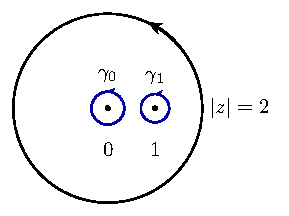
\includegraphics[width=.45\linewidth]{figs/fig08-02-contour-deformation.pdf}
\caption{Deforming the large circle into two positive circles about the singularities.}
\label{fig:fig08-02-contour-deformation}
\end{figure}


The integral on $\gamma_1$ is $2\pi \mathrm{i} e$. To evaluate the one on $\gamma_0$,
choose $|z|=\rho<1$ and use
\begin{equation}\label{eq:14}
e^{1/z}=\sum_{m=0}^{\infty}\frac{z^{-m}}{m!},
 \qquad
 \frac1{z-1}=-\sum_{k=0}^{\infty}z^k.
\end{equation}
Both series converge absolutely and uniformly on this fixed circle. Their
product may therefore be integrated term by term. The coefficient of
$z^{-1}$ is
\begin{equation}\label{eq:15}
-\sum_{k=0}^{\infty}\frac1{(k+1)!}=1-e.
\end{equation}
The contour moments above now give
\begin{equation}\label{eq:16}
\oint_{\gamma_0}\frac{e^{1/z}}{z-1}\dd z=2\pi \mathrm{i}(1-e),
 \qquad
 \boxed{\oint_{|z|=2}\frac{e^{1/z}}{z-1}\dd z=2\pi \mathrm{i}.}
\end{equation}
These series calculations anticipate the power-series and Laurent-series
methods discussed in Lectures 8 and 9.

\subsection{A contour with an inner boundary}
Let $C_{\mathrm{out}}$ and $C_{\mathrm{in}}$ be counterclockwise circles
$|z-1|=3/2$ and $|z-1|=1/2$. The positive boundary of the intervening
annulus is
\begin{equation}\label{eq:17}
C=C_{\mathrm{out}}-C_{\mathrm{in}}.
\end{equation}
Thus the inner boundary is traversed clockwise. For this orientation,
consider
\begin{equation}\label{eq:18}
K=\oint_C\frac{e^{1/z}}{z^2-1}\dd z.
\end{equation}


\begin{figure}[htbp]
\centering
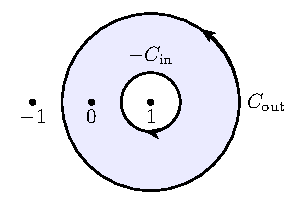
\includegraphics[width=.48\linewidth]{figs/fig08-03-annular-boundary.pdf}
\caption{Positive boundary of the annulus: the outer circle is counterclockwise and the inner circle is clockwise.}
\label{fig:fig08-03-annular-boundary}
\end{figure}


Only $0$ lies in the annulus: $1$ is in the hole and $-1$ is outside the
outer circle. Deformation reduces $K$ to a small positive circle about $0$.
On $0<|z|<1$,
\begin{equation}\label{eq:19}
\frac{e^{1/z}}{z^2-1}
 =-\left(\sum_{m=0}^{\infty}\frac{z^{-m}}{m!}\right)
      \left(\sum_{k=0}^{\infty}z^{2k}\right).
\end{equation}
The coefficient of $z^{-1}$ is
$-\sum_{k=0}^{\infty}1/(2k+1)!=-\sinh1$, so
\begin{equation}\label{eq:20}
\boxed{K=-2\pi \mathrm{i}\sinh1.}
\end{equation}
Reversing this whole boundary changes the sign. If instead both circles
are traversed counterclockwise, the contour is $C_{\mathrm{out}}+
C_{\mathrm{in}}$, and its integral is $2\pi \mathrm{i}\cosh1$.

\section{Taylor Expansion: Example 4.15}
Consider $f(z)=1/z^3$ and expand about $z_0=1$.

The nearest singularity is $z=0$, at distance $1$. Direct differentiation
gives
\begin{equation}\label{eq:21}
f^{(n)}(1)=\frac{(-1)^n(n+2)!}{2},
 \qquad
 \boxed{\frac1{z^3}=\sum_{n=0}^{\infty}
       (-1)^n\frac{(n+1)(n+2)}2(z-1)^n,\quad |z-1|<1.}
\end{equation}
An indirect method begins with
\begin{equation}\label{eq:22}
\frac1z=\frac1{1+(z-1)}
       =\sum_{n=0}^{\infty}(-1)^n(z-1)^n,\qquad |z-1|<1.
\end{equation}
Since $(1/z)''=2/z^3$, differentiate twice and divide by $2$:
\begin{equation}\label{eq:23}
\frac1{z^3}
 =\frac12\sum_{n=2}^{\infty}(-1)^n n(n-1)(z-1)^{n-2}
 =1-3(z-1)+6(z-1)^2-10(z-1)^3+\cdots .
\end{equation}

\section{Assigned Exercises}
Textbook p.~83: B8--B10; p.~116: A1, A2, A4 and B1--B2.
Use the assigned subitems for A1 and A2.

\section{Checks on the Calculations}
The factorization
\begin{equation}\label{eq:24}
5\zeta-2\zeta^2-2=-2(\zeta-\tfrac12)(\zeta-2)
\end{equation}
changes the prefactor $2/\mathrm{i}$ to $-1/\mathrm{i}$. This gives
$4\pi/3$ for the arc-length integral.

For an annular region, the positive inner boundary is clockwise. The
value $-2\pi\mathrm{i}\sinh1$ uses that boundary orientation. It changes
sign if the whole boundary is reversed.

The identity $(1/z)''=2/z^3$ has a positive sign. It gives the coefficients
$1,-3,6,-10,\ldots$ in the Taylor expansion of $1/z^3$ about $1$.

\end{document}
